\documentclass[11pt,twocolumn]{article}

\usepackage[a4paper, margin={.5in, .5in}]{geometry}
\usepackage{latexsym,graphicx}
\usepackage{amsmath,amssymb}
\usepackage{amsthm}
\usepackage{enumerate}
\usepackage{graphicx}
\usepackage{cleveref}
\usepackage{algorithmic}
\usepackage{algorithm}

% Useful macros
\newcommand{\E}[1]{\mathbf{E}\l[#1\r]}
\newcommand{\problem}[1]{\section*{Problem #1}}
\renewcommand{\l}{\left}
\renewcommand{\r}{\right}
\renewcommand{\iff}{\Leftrightarrow~}
\newcommand{\intff}{\int_{-\infty}^\infty }
\newcommand{\intzf}{\int_0^\infty }
\newcommand{\intpp}{\int_{-\pi}^\pi }
\newcommand{\sumzf}[1]{\sum_{#1=0}^\infty}
\newcommand{\sumff}[1]{\sum_{#1=-\infty}^\infty}
\newcommand{\Bin}{\text{Bin}}
\newcommand{\pfrac}[2]{\l(\frac{#1}{#2}\r)}
\renewcommand{\bf}{\textbf}
\newcommand{\zm}[1]{z^{-#1}}
\renewcommand{\P}[1]{\mathbf{P}\l\{#1\r\}}
\newcommand{\Var}[1]{\mathbf{Var}\l(#1\r)}
\newcommand{\Poiss}{\text{Poiss}}
\newcommand{\Geom}{\text{Geom}}
\newcommand{\Skew}{\text{\bf{Skew}}}

\newtheorem{lemma}{Lemma}
\newtheorem{theorem}[lemma]{Theorem}
\newtheorem{informaltheorem}[lemma]{Informal Theorem}
\newtheorem{informallemma}[lemma]{Informal Lemma}
\newtheorem{corollary}[lemma]{Corollary}
\newtheorem{definition}[lemma]{Definition}
\newtheorem{proposition}[lemma]{Proposition}
\newtheorem{question}{Question}
\newtheorem{example}[lemma]{Example}
\newtheorem{remark}[lemma]{Remark}
\newtheorem{claim}{Claim}
\newtheorem{fact}{Fact}
\newtheorem{challenge}{Challenge}
\newtheorem{observation}{Observation}
\newtheorem{openproblem}{Open Problem}
\newtheorem{openquestion}{Open question}
\newcommand{\todo}[1]{\noindent \colorbox{green}{\begin{minipage}{\linewidth}{\bf TODO:} #1\end{minipage}}}

\newcommand{\beq}{\begin{equation}}
\newcommand{\eeq}{\end{equation}}
\newcommand{\beas}{\begin{eqnarray*}}
\newcommand{\eeas}{\end{eqnarray*}}

\newcommand{\poly}{\mathrm{poly}}
\newcommand{\eps}{\epsilon}
\newcommand{\e}{\epsilon}
\newcommand{\polylog}{\mathrm{polylog}}
\newcommand{\rob}[1]{\left( #1 \right)} %Round Brackets
\newcommand{\sqb}[1]{\left[ #1 \right]} %square Brackets
\newcommand{\cub}[1]{\left\{ #1 \right\} } %curly brackets
\newcommand{\rb}[1]{\left( #1 \right)} %Round
\newcommand{\abs}[1]{\left| #1 \right|} %| |
\newcommand{\zo}{\{0, 1\}}
\newcommand{\zonzo}{\zo^n \to \zo}
\newcommand{\zokzo}{\zo^k \to \zo}
\newcommand{\zot}{\{0,1,2\}}
\newcommand{\norm}[1]{\left\lVert#1\right\rVert}
%
%\newcommand{\en}[1]{\marginpar{\textbf{#1}}}
%\newcommand{\efn}[1]{\footnote{\textbf{#1}}}
\newcommand{\bR}{\mathbb{R}}
\newcommand{\bE}{\mathbb{E}}

%%%%%%%%%%%%%%%%%%%%%%%%%%%%%%%%%%%%%%%%%%%%%%%%%%%%%%%%%%%%%%%%

\begin{document}

\section{Introduction: Distributed informations Systems, an Overview}


\subsection{Information System}

An information system is a \bf{software} that manages a \bf{model} of some aspect of the \bf{real world} within a (distributed) computer system for a given \bf{purpose}.
\\
\\
We can identify 3 types of real world aspect:
\begin{itemize}
	\item \bf{Physical phenomena:} measure the environment and create models of physical phenomena: meteorological IS, geo IS,...
	\item \bf{Social organization:} capture the roles, relationship activities, ... in social organization such as business and institutions.
	\item \bf{Human thought:} model human thought and reasoning processes. Capture the meaning of texts and other media, assess the importance and quality of information but also model human traits such as sentiments or opinion.
\end{itemize}

\subsubsection{Model}
Mathematical structure consisting of a set of:
\begin{itemize}
\item \bf{Constant} (or identifier)
\item \bf{Function} (or relation)
\item \bf{Axioms} (or constraint)
\end{itemize}
Example of model: a physical phenomena:

\begin{itemize}
\item Constant: coordinate values, temperature values
\item Function: T(x,y) $\rightarrow$ return temperature for a given coordinate.
\item Axiom: $-60 < T(x,y) < 60$
\end{itemize}
A function can be represented:

\begin{itemize}
\item Implicitly: $f(x) = x^2$
\item Explicitly: $f(1) = 1, f(2) = 4, f(3) = 9$ also called \bf{data}
\end{itemize}
Information system strongly emphasize \bf{explicit} representation, because many aspect of the world are not algorithmically defined: birthdate of a person. \bf{Implicit} representation play nevertheless an important role for queries, view, user definition functions
\\
\\
A model is linked by an \bf{interpretation or relationship} to the real world $\rightarrow$ maps every constant of the model to some real word object and the function preserve all relationship that occur in the real world. The interpretation relationship is \bf{homomorphic}. 

\begin{figure}[!ht]
\begin{center}
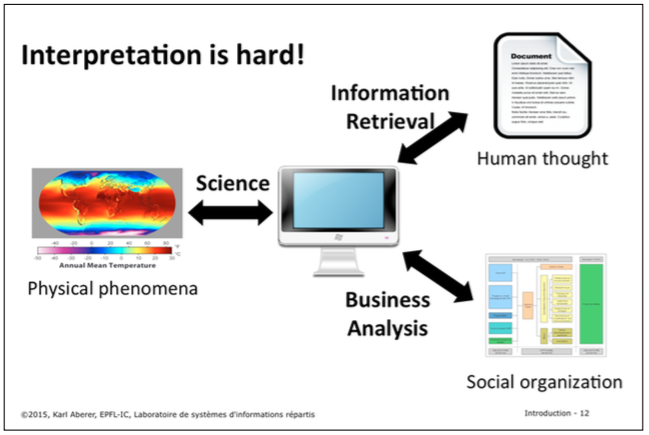
\includegraphics[width=1\linewidth]{figures/interpretation_hard.png}
\end{center}
\caption{interpretation is hard}
\end{figure}

Interpretation is hard because there is no way to formally verify function in the real world

\subsubsection{Data Management}
 \bf{Data model}: used to represent a model in a computer system. A data model D uses \bf{data structure} (associative array, labelled graphs, relational tables) and \bf{operation} (add(k,v), search(key),...) for the representation of the constants, data, and constraint of a model within a computer system.
 
 
 \paragraph{Database}: The collection of data represented in a data model D


\paragraph{Database Management System DBMS:} is a computer system designed to manage database. DBMS can be used to manage databases an this realize IS. The inverse is not necessarily true. 
\\
\\ Data Model is interchangeable used to represent two different things:

\begin{itemize}
	\item Data model used to represent a model within 	a computer system (sense we will use)	
	\item A formalism to specify a whole class of data model e.g; relational data model. Data modelling formalism consists of two part:
	
	\begin{itemize}
		\item \bf{Data definition model (DDL):} enables the specification of data models, consisting of possible data structure and integrity constraints. Specification of a data model using DDL is called \bf{database schema or schema}. Example \textit{CREATE TABLE student ... PRIMARY KEY}
		\item \bf{Data Manipulation language (DML):} allow to specify function in the data model. Ex: \textit{SELECT name FROM ...}
	\end{itemize}
\end{itemize}
Data Modelling formalism has 3 main component:

\begin{itemize}
	\item \bf{Data Structures:} collection of data structures which are used to represent database
	\item \bf{Integrity Constraints:} a language to express rules the data in database has to observe
	\item \bf{Manipulation:} a collection of operations which can be applied to the data structure to update, transform and query the data in the DB
\end{itemize}

\paragraph{Database Management System} is the software that implement a data modelling formalism ( MySql, PostgreSQL, Microsoft access, SQL Server, FileMaker, Oracle, but \bf{not} XML).

\paragraph{Logical Data Independence:} the same data can be viewed in different ways:
\begin{itemize}
	\item Views compute different data model on top of the same data stored in a database
	\item Corresponds to different model based on the same data (ex: university ranking, same data but each one find a different rank)
\end{itemize} 

\paragraph{Database Systems:} an IS based on a DBMS. The information system is concerned with providing a model for real world aspect, whereas the database system is concerned with the \bf{efficient management of the data structure required to represent the model}



\subsubsection{Data management Tasks}
2 challenges:
\begin{itemize}
	\item \bf{Efficient} management of large amounts of data (storage(column vs Row), indexing(B+- tree), search, aggregation)
	\item safety of the data: \bf{persistence } and \bf{consistency} of data under updates and failure (independent of lifetime of programs and type of failure)
\end{itemize}
Optimizing access to database:

\begin{itemize}
	\item \bf{Physical database design:} choice of the data structures and storage layout that match best the requirement of applications. Choice performed before the accesses to the database are executed
	\item \bf{Declarative Query Optimization:} choice of the best algorithm, given some storage and indexing scheme, when a concrete operation such as query is to be executed. Performed at the time the access to the database is executed
\end{itemize}
Transaction Management:

\begin{itemize}
	\item \bf{Isolation} others users do not influence own transaction
	\item System failure do not affect the execution of operations:
	\begin{itemize}
		\item \bf{Atomicity:} transaction are completely executed or not at all
		\item \bf{Durability:} once transactions are executed their results are never lost
	\end{itemize}
\end{itemize}

\paragraph{Physical Data Independence:}  concept that the same logical database ( having the same database schema) can be physically realized in many different way (using different physical database design) and the same logical operation (query, update) can be executed in physically different way using declarative query optimization and transaction management. 


\paragraph{Modeling architecture}: defined as standard by ANSI:
\begin{itemize}
	\item \bf{Conceptual Schema or Semantic layer:} Domain specific abstract models
	\item \bf{Logical Schema or semantic layer:} Data models
  	\item \bf{Physical Schema:} Physical storage on disk, in the network
\end{itemize}

\subsubsection{Information Management}
Between data and models:
\begin{itemize}
	\item \bf{Retrieval:} from models to data: given a model of reality we would like to learn about specifics aspect of reality
	\item \bf{Data mining:} from data to model: given a data find a model that match the data
\end{itemize}
Between model and real world:
\begin{itemize}
	\item \bf{Conceptual modeling:} From real world to Model: analyze the real world and specify a model
	\item \bf{Evaluation:} From model to real world: given a model evaluate it against reality.
\end{itemize}
Between data processing system and real world:
\begin{itemize}
	\item \bf{Control:} from data to real world: data generated can in the IS can be used to control real device
	\item \bf{Monitoring} from real world to data: the real world generate data that can be processed in the IS
\end{itemize}

\begin{figure}[!ht]
\begin{center}
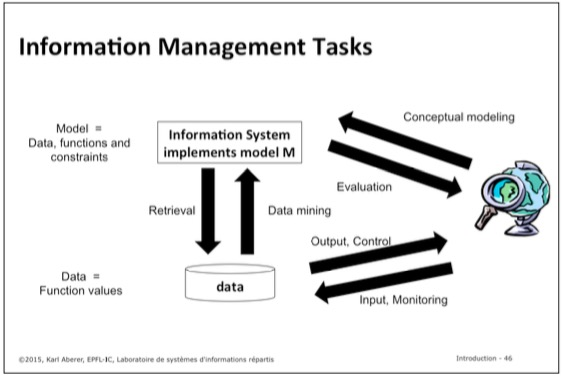
\includegraphics[width=1\linewidth]{figures/informationManagementTasks.jpg}
\end{center}
\caption{Information management tasks}
\end{figure}

\paragraph{Utility of information:} depend on:
\begin{itemize}
	\item \bf{Nature/Importance} of the decision
	\item \bf{Quality} of the decision
\end{itemize}

\begin{figure}[!ht]
\begin{center}
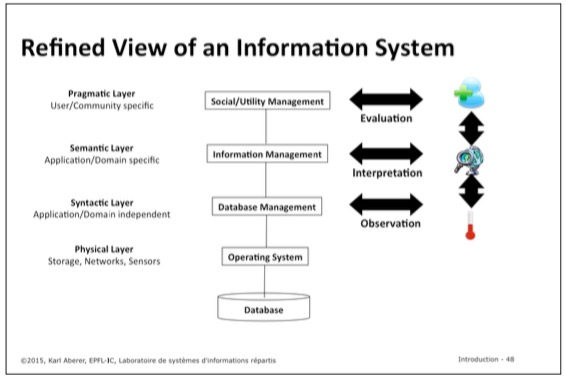
\includegraphics[width=1\linewidth]{figures/viewIS.jpg}
\end{center}
\caption{Overview of an information system}
\end{figure}

\subsection{Distributed information system}
\begin{itemize}
	\item \bf{Distributed data management:} use of distributed physical resources: locality of access, scalability, parallelism in the execution
	\item \bf{Heterogeneous information system:} use of different data models to represent the same information and different access methods. We have to deal with each IS are under the control of different \bf{Autonomous authorities:} $\Rightarrow$ independent users have to collaborate, coordinate, negotiate to perform information management task
\end{itemize}

\subsubsection{Distributed Data Management}
\begin{itemize}
\item \bf{Data Partitioning:} move the data to the nodes in the network where it is mostly used
\item \bf{Distributed Query Processing:}  deals with the problem of analysing queries and deciding which data can retrieved from which node
\item \bf{Data Replication:} replicate data if frequently used on different node $\oplus$ improves data access $\ominus$ update more expensive, consistency
\item \bf{Data Caching:} keep a copy of the data when transmitted in a network
\end{itemize}

\paragraph{Control:}
\begin{itemize}
\item \bf{Push access:} add new profile in database for example
\item \bf{Pull access:} query a specific profile for example
\end{itemize}


\paragraph{Communication model:}
\begin{itemize}
\item \bf{Unicast:} p2p connection
\item \bf{Multicast:} propagate requests to multiple receivers. example:\bf{Gossiping protocol:} sends request to local neighbourhood, then this neighbour spread the message,... until some peer can respond to the request
\item \bf{Broadcast:} send the request to all clients that are listening
\end{itemize}

\paragraph{Event:}
\begin{itemize}
\item \bf{Periodic:} periodic
\item \bf{Conditional:} on change(update)
\item \bf{Ad-hoc:} request by application or users (correspond to traditional client-server model)
\end{itemize}

\subsubsection{Heterogeneity}
\paragraph{Semantic heterogeneity:} the same real world aspect can be modelled differently. relating different models requires human intervention : human attention is a scare resource!

\paragraph{Solution: Mapping:}
\begin{itemize}
\item \bf{Standardization:} mapping through standard
\item \bf{Ontologies:} Mediated mapping. relate the model of an information system to a common model and use this mapping to construct a direct mapping among the different models used in the information systems\\
\item \bf{Mapping:} Direct mapping among two information system
\end{itemize}

\paragraph{Syntactic heterogeneity:} the same data can be represented using different data models (relational vs xml)

\begin{figure}[!h]
\begin{center}
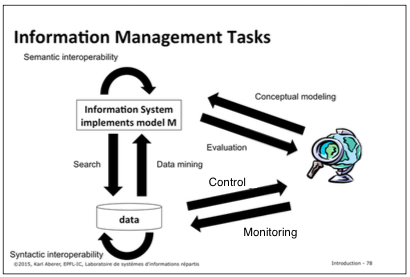
\includegraphics[width=1\linewidth]{figures/informationManagementTasks2.png}
\end{center}
\caption{Information management tasks}
\end{figure}


\subsubsection{The User Problem}
\begin{itemize}
\item bf{Trust:}Can I trust the information I received?
\item \bf{Privacy:} Can I trust the user to use my information I sent correctly
\end{itemize}
The \bf{more quality information} we reveal the \bf{more trust} we may expect, but the \bf{more} we also put out \bf{privacy} in danger.

One way to evaluate the quality of information, and thus the level of trust we can have in a user providing information, is to share recommendations with other users on how they perceive the quality of this information

\begin{figure}[!ht]
\begin{center}
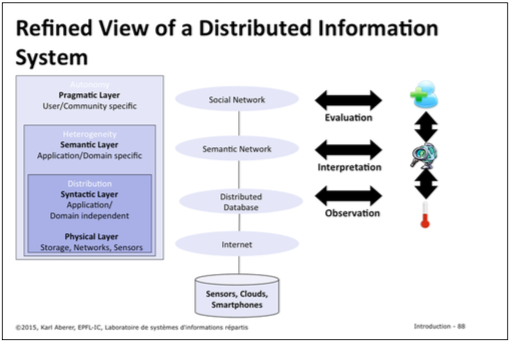
\includegraphics[width=1\linewidth]{figures/viewIS2.png}
\end{center}
\caption{Overview of an information system}
\end{figure}







\section{Knowledge Modeling - Graph Databases}
The goal is to turn schema-less data into data with schema by exploiting the embedded schema information and identifying the structural regularities in a given database. 

\subsection{Graph Data Model}
The graph data model is used as it can generalize common data models (e.g. relational, XML, RDF, etc).
\subsubsection{Formal Definition} 
\includegraphics[width=1\linewidth]{figures/data_graph.png}
\begin{itemize}
  \item Data graph: D = (V, E, R) is a labeled, rooted and directed graph 
  \item V is a set of nodes
  \item E $\subseteq$ V x L x V is a set of labeled edges, they determine the meaning of the data values stored in the leaves
  \item R $\subseteq$ V is a set of root nodes that have no incoming edges. All nodes in V are reachable from some root in R
  \item A $\subseteq$ V are the atomic nodes = set of leaf nodes storing typed data values
  \item C $\subseteq$ A x U x T is the data stored in D, where U is the domain of all data values and T are the data types
\end{itemize}

\subsubsection{Structural Properties}
We can enumerate the paths starting from the root to capture the structure of the data graph. A possible schema would be to use a \textbf{trie} enumerating those paths and labeling the leaf nodes with the data type that is found in the graph database. However, it contains many redundant structures so it would be better to combine different subgraphs into a common graph structure. 

\subsubsection{Simulation and Schema Graphs}
Simulation is used to provide a criterion to decide whether a schema graph S correctly captures the structure of a data graph D. A schema graph may use alternate labels or wildcards on edges. Condition: for every node d in D reached by a path p starting from the root there exists a corresponding node s in S reachable by the same path and the types of the leaf nodes are the same in case d is a leaf node. S simulates D is denoted as D $<$ S.

More formal definition of the simulation relationship among labelled graphs:
\begin{itemize}
  \item Given graphs G$_{1}$, G$_{2}$ and relation R $\subseteq$ V$_{1}$ x V$_{2}$, then R is a simulation if for all labels l $\in$ L and for all x$_{1}$, y$_{1}$ $\in$ V$_{1}$ and for all x$_{2}$ $\in$ V$_{2}$ it holds that if x$_{1}$ $\rightarrow$$_{l}$ y$_{1}$ and R(x$_{1}$, x$_{2}$) then there exists y$_{2}$ $\in$ V$_{2}$ such that R(y$_{1}$, y$_{2}$) and x$_{2}$ $\rightarrow$$_{l}$ y$_{2}$
  \item If it holds, G$_{2}$ simulates G$_{1}$ and we can write G$_{1}$ $<$ G$_{2}$
\end{itemize}

We have to extend the concept of simulation relationship for the graph data model:
\begin{itemize}
  \item A schema graph S is a schema for a data graph D if there exists a rooted, typed simulation of D using S (that may contain wildcards and alternate labels). We require that root and leaf nodes in the data graph are related to root and leaf nodes in the schema graph. 
  \item Rooted simulation: R(r$_{1}$, r$_{2}$) for the roots r$_{1}$ and r$_{2}$  
  \item Typed simulation: for all x, y if R(x, y) and y is an atomic type then x must be an atomic node with content of that type
  \item For wildcards and alternate labels the label in the data graph has to be contained in the set of labels specified by these extended schema edge labels: if x$_{1}$ $\rightarrow$$_{l}$ y$_{1}$ then x$_{2}$ $\rightarrow$$_{l}$ y$_{2}$ or x$_{2}$ $\rightarrow$ $_{\_}$ y$_{2}$ or x$_{2}$ $\rightarrow$$_{l|k|...}$ y$_{2}$

\end{itemize}

\subsubsection{Classification by Schema Graphs}
We can define the rooted simulation R as a table with S nodes on the left (Class) and corresponding nodes in D on the right (Instances). The database schema classifies the data in the database.

\paragraph{Multiple classification}A data node may belong to multiple classes. Two different valid simulations could classify the same data node in different classes (as it requires to be classified in at least one class, but not all possible classes), which could lead to ambiguous classification.

\paragraph{Maximal simulations}It guarantees that the resulting classification is unique. Given two simulations R$_{1}$ and R$_{2}$ between a data graph and a schema graph the following holds: D $<$$_{R1}$ S and D $<$$_{R2}$ S then  D $<$$_{R1 \cup R2}$ S. The maximal simulation can be computed as a fixpoint iteration. (For small graphs, we can simply check for each node of the data graph if it could be added to the schema graph, for example leaves should remain leaves and for the other nodes the same outgoing/ingoing edges and paths)

\paragraph{Fixpoint iteration}We start from the total relation between all nodes of D and S, i.e., data instances belong to all classes. Then we stepwise eliminate those pairs in R that violate the simulation condition. That is, whenever a pair should be contained in R we check whether a corresponding link exists in the data graph.
\begin{algorithm}
\caption{Fixpoint iteration for data graph D, schema graph S}
\begin{algorithmic} 
\STATE $R' \leftarrow \emptyset$
\STATE $R \leftarrow \{ (o, c) | o \in D, c \in S \}$
\WHILE{$R \neq R'$}
\STATE $R' \leftarrow R$
\STATE $R \leftarrow  \{ (o, c) |$ all $(o, c)$ such that either o is atomic value and c its type or there exists $(o', c') \in R'$ and $o \rightarrow _{l} o' \in D$ and $c \rightarrow _{l} c' \in S \}$
\ENDWHILE
\end{algorithmic}
\end{algorithm}

\subsubsection{Refining Schemas}
\begin{itemize}
\item Refinement is needed when a schema evolves and becomes more precise over time as more information on the databases become available. 
\item We say that schema S$_{1}$ subsumes schema S$_{2}$ if S$_{1}$ contains less detail and is more general than schema S$_{2}$. It implies that all databases that conform to S$_{2}$ also conform to S$_{1}$
\item This is the case if S$_{2}$ $<$ S$_{1}$. So if S$_{2}$ is a schema for D (D $<$ S$_{2}$) then we can conclude that D $<$ S$_{1}$ and therefore S$_{1}$ is also a schema for D.
\end{itemize}

\subsection{Schema Extraction}
The goal is to automatically construct a schema graph from the data graph. 
\subsubsection{Data Guide}
The resulting schema graph should be:
\begin{itemize}
\item \textbf{Accurate}: every path that occurs in the schema graph occurs in the data graph and vice versa
\item \textbf{Concise}: every path occurs only once
\end{itemize}
It is called a \textbf{data guide}. Data guide nodes correspond to subsets of data graph nodes. Its root node is the set containing the data graph root. 

\paragraph{Data Guide Construction}
For each data guide node constructed and for each edge label of an  edge leaving in the data graph some element from the data guide node:
\begin{itemize}
\item form the set of nodes in the data graph reached by this edge label
\item if the set exists already in the data guide, create a labeled edge to it
\item else create a new data guide node and connect it by the edge
\end{itemize}
Continue until no more new data guide nodes are created.
\\
\includegraphics[width=1\linewidth]{figures/data_guide.png}
\paragraph{Properties}
\begin{itemize}
\item Same nodes of data graph occur in multiple places $\rightarrow$ space complexity! Problem: node equivalence (if the paths leading to two nodes in the data graph are the same, the nodes are equivalent)
\item Repeating structures in the data graph are reduced to a single structure in the data guide (less edges)
\item Sometimes it can be more complex than the data graph itself
\item Deterministic graph = DFA. It is minimal, deterministic schema graph with 1:1  correspondence among data guide nodes and sets of nodes reached by the  same paths (strong dataguide)
\item Cycles in the data graph lead to cycles in the data guide
\end{itemize}

\paragraph{Semistructured Data Indexing}
As the data guide is deterministic we can use it as an indexing structure (each data guide node stores for each label the data guide node reached by the label and the graph database nodes). Answering a query is simple:
\begin{itemize}
\item for a non-terminal query element look-up the next data guide node
\item for a terminal element look-up the graph database nodes
\end{itemize}

\subsubsection{Language Equivalence}
To overcome the space complexity of data guides, non-deterministic schema graphs could be used. We can observe that if the set of paths leading to two nodes in the data graph are the same, the nodes are equivalent from the viewpoint of query processing. Formal definitions:
\begin{itemize}
\item Language: set of all possible paths to node x. L$_{x}$ = {p = p$_{1}$..p$_{n}$ p is a path from the root to x}
\item Language equivalent nodes: x $\equiv$ y if L$_{x}$ = L$_{y}$
\item Equivalence class of x denoted as [x]
\end{itemize}
Then we can create one node for language equivalent nodes. 
Drawback: checking for language equivalence is pspace complete. Solution: approximate language equivalence by a computationally more feasible relation. 

\paragraph{Approximation}A relation $\approx$ is an approximation of $\equiv$ if $\forall$ x,y: x $\approx$ y $\rightarrow$ x $\equiv$ y. 
\\
Queries will be correctly answered but query evaluation will be more expensive as there are more nodes to be checked. The reverse bisimulation is such a relationship. 

\paragraph{Reverse Bisimulation}
\begin{itemize}
\item It is equivalent to the simulation relation in both directions with the edges of the graphs inverted
\item On any graph there exists a maximal reversed bisimulation relation which can be efficiently computed and $\forall$ x,y: x $\approx$ y $\rightarrow$ x $\equiv$ y
\item If x $\approx$ y and x is the root then y is the root, and vice versa. If x $\approx$ y and there exists an edge x' $\rightarrow$$_{l}$ x then there exists an edge y' $\rightarrow$$_{l}$ y and x' $\approx$ y', and vice versa. 
\end{itemize}

\paragraph{Index Construction} 
\begin{itemize}
\item Every equivalence class is one node of the index graph. The nodes are connected with a labeled edge if such an edge exists between the members of the equivalence class in the data graph. 
\item This is an \textbf{unambiguous} definition since the equivalence classes cannot be distinguished from the viewpoint of accessibility through paths (either all members of two equivalence classes are connected by a labeled edge or none, otherwise the classes would be different).
\item Query processing will in general have to follow multiple paths in the non-deterministic data guide.
\item The index cannot be larger than the database itself.
\item The hash table for a node contains the key (label of outgoing edge), the corresponding index graph node and the data graph nodes for this index.
\end{itemize}

\subsection{Schema Mapping}
The goal is to integrate data that are available in two graph databases and that are semantically related to each other. So given two graph schemas S1 and S2 with two graph databases D1 and D2 we need to find a 1:1 matching of schema nodes (classes) that have the same or similar meaning (same or similar instances). Issue: D1 and D2 might have different extensions.

\subsubsection{Jaccard Similarity}
We can measure the level of similarity at the content level using the Jaccard Similarity. Let U be the finite set of possible instances, A and B classes which are subsets of U. 
\[
  sim(A,B) = \frac{|A \cap B|}{|A \cup B|} = \frac{P(x \in A \land x \in B)}{P(x \in A \lor x \in B} = \frac{P(A,B)}{(P(A,B)+P(\bar{A},B)+P(A,\bar{B}))}
\]
We can notice that if A has leaf nodes and the instances of B are complex data the similarity would be 0 even if B contains the same instances as A at the leaf level, that's why we introduce the features of classes.

\subsubsection{Features of Classes}
Content feature = set of terms associated with the paths of a node $i$ to the leaves with repeated occurrences $T_{i} = \{t_{1},...,t_{n}\}$, simply all the leaves from a node $i$.

\subsubsection{Probabilistic Approach: Naive Bayes Classifier}
Directly comparing the features does not always help to detect the correspondences as due to different database extensions and different naming conventions, even classes that have a strong semantic similarity often have no common instances in two different databases. We may assume that $U1 \cap U2 = \emptyset$.
\\
We cannot compute P(A,B) directly. A better approach would be: given $i \in B$ would be likely that also $i \in A$, even if $i$ is not part of U1. We can construct a function that gives the probability for a given instance $i$ with feature $T_{i}$ to belong to a class A, using Bayes law:
\[
  P(A|T_{i}) = P(T_{i}|A)P(A)
\]
This is the Na�ve Bayes Classifier.
\\
We know that:
\begin{itemize}
\item $P(A) = \frac{|A|}{|U_{1}|}$ 
\item $P(t_{i}|A) = P(t_{1}|A)...P(t_{n}|A)$, by independence assumption 
\item $P(t|A) = \frac{|t \in T_{A}|}{\sum_{t'}{|t' \in T_{A}|}}$ 
\end{itemize}

\subsubsection{Steps to compute similarity between classes A and B}
\begin{itemize}
\item take all instances of U1 and train a classifier to decide whether an instance belongs to A or not
\item take all instances in U2 and split into U2$^{B}$ and U2$^{\bar{B}}$
\item apply the classifier trained with U1 to all instances in U2 to produce sets U2$^{AB}$,  U2$^{A\bar{B}}$,  U2$^{\bar{A}B}$
\item do the same with the roles of U1 and U2 inverted
\item compute $P(A,B) = \frac{|U1_{AB}|+|U2_{AB}|}{|U1|+|U2|}$, same for $P(A, \bar{B})$, etc.
\item compute for each pair of concepts sim(A,B) using Jaccard Similarity.
\end{itemize}
Instead of taking instances as a whole, we can tokenize the instance's name and compute P(word|concept). 
\subsubsection{Node Mapping}
Having the similarity values, alternative class mappings are possible. A naive approach: first the best matches are used to produce mappings, then the mapped classes are removed (to assure that each class is mapped to a unique other class) and then the process continues.


% Sebastien S
\section{Clustering and classifications}

\subsection{Clustering}
\textbf{The main idea:} Given a dataset of objects described by attributes, build a model that assigns objects to a class. 

\begin{itemize}
	\item \textbf{produces classes} which are not know in advance (called clusters)
	\item objects that belong to the same cluster are similar
	\item said \textbf{unsupervised} since objects do not have class information 
	\item serves for exploratory data analysis with little or \textbf{no prior knowledge}
\end{itemize}

\subsubsection*{Issues with clustering}

\begin{itemize}
	\item high-dimensional data is too sparsely distributed 
	\\ $\rightarrow$ project data into a lower dimensional space
	\item many methods can detect only very simple geometrical sphapes
\end{itemize}

\subsubsection*{Partitioning methods}
Given dataset $D$ of $n$ objects, partition it into k sets $S_1, ..., S_k$. The goal of this method is to minimise the cost function $J$. 
Optimal algorithm isn't practical. There exists different heuristic algorithms:

\begin{itemize}
	\item \textbf{K-means}: cluster is represented by the point whose mean distance with the objects in the cluster is minimal

	\item \textbf{K-medoids}: cluster is represented by the object whose mean distance with the objects in the cluster is minimal

	\item \textbf{K-medians}: cluster is represented by the point whose median distance with all the objects in the cluster is minimal
\end{itemize}
Here is $J$'s formulation for the K-means algorithm:
\begin{align*}
	J = \frac{1}{n} \sum_{i = 1}^{k} \sum_{x_j \in S_i} || x_j - \mu_i ||^2 , \quad \mu_i = \frac{1}{|S_i|} \sum_{x_j \in S_i} x_j
\end{align*}

and the algorithm:

\noindent

\begin{enumerate}
	\item randomly init the prototypes $\mu_i$
	\item assign each object to the nearest prototype
	\item update prototypes $\rightarrow$ put them in the middle of their cluster
	\item update objects assignements (again to the nearest prototype)
	\item if it hasn't converged, then go back to step 3.
\end{enumerate}
Some issues with K-mean:
\begin{itemize}
	\item often terminates at local optimum
	\item need to specify the number of cluster in advance
	\item do not handle outliers
	\item only has convex shapes
\end{itemize}
There exists other methods which do not suffer from these issues:
\begin{itemize}
	\item Hierarchical clustering: starts with $n$ clusters and then iteraticely merge them if there are similar.

	\item Density-based clustering: discover clusters of arbitrary shape by checking if the number of objects in the neighnourhood of a given objet is above a certain density threshold

	\item Online incremental clustering: place each new incoming object into an existing cluster or a new one.
\end{itemize}


\subsection{Classification}
\textbf{The main idea:} Starting with a given classification of data items and their attributes, predict the membership to a specific class of a new data object.

\begin{itemize}
	\item said \textbf{supervised} since it is based on existing data
	\item useful in decision problems, where for a given data item a decision is to be made
	\item the model is a function that return the class label fiven the remaining attributes of an unknown object
	\item the classes are known
\end{itemize}

A good model classifies accurately the items in the training set and generalises well for the unknown items in the test set.

\subsubsection*{Decision tree}
In a decision tree, at each level, one of the existing attributes is used to partition the data set based on the attribute value. In such a tree, leaves represent the calues of the class label.

Generally a decision tree is constructed in a top-down manner by recursively splitting the training set using conditions on the attributes. First, all data objects are assign to the root and, based on selected attributes, objects are partitioned. The recursion stops when all samples belong to the same class or if there is no attributes left. In a second phase, we remove leaves correpsonding to outliers.

The attribute selection is based on the amount of entropy in the set S ar a given branch in the tree, defined by:
\begin{align*}
	H(P, N) = - \frac{P}{P + N} \log_2 \frac{P}{P + N} - \frac{N}{P + N} \log_2 \frac{N}{P + N} 
\end{align*}
with $P$ and $N$ the number of positive and negative samples respectively. The mount of information needed to classify the data after the split according to attribute $A$ is obtained by calculating $H(p,n)$ for each of the partitions and weightting these values by the probability that a data item belongs to the respective partition.

\begin{align*}
	H(A) = \sum_{i = 1}^v \frac{P_i + N_i}{P + N} H(P_i, N_i)
\end{align*}
with $A$ partitioning $S$ into $S_1, ..., S_v$ and $P_i$, $N_i$ the number of respectivelty positive or negative samples in $S_i$.

The information gained (reduction of uncertainty) by a split is given by

\begin{align*}
	Gain(A) = H(P, N) - H(A)
\end{align*}

We then just have to take the attribute that leads to the highest reduction of uncertainty. However, it is important to understand that for a test dataset, a classifier might overspecialize and capture noise and outliers in the data rather than general properties. A first strategy to overcome this problem could be to stop partitioning when some criteria is met like the number of samples assigned to a leaf node

Another idea is to use the principle of \textbf{minimum description length}.
\begin{itemize}
	\item Let $M_1, M_2, ..., M_n$ be a list of candidate models. The best model is the one that minimizes
	$$ L(M) + L(D | M) $$

	\item $L(M)$ is the length in bits of the description of the model ($\#$nodes, $\#$leaves,...)
	\item $L(D|M)$ is the length in bits of the description of the data when encoded with the model
\end{itemize}

In a second phase, using a efficiency measurement of the tree nodes (count the number of mislassifications), we can merge some of the leaves. \\
Decision trees issues:
\begin{itemize}
	\item extremely sensitive to small perturbations in the data and not incremental. A slight change or some new data available implies that the whole tree must be reconstructed from scratch.
	\item easily overfits
\end{itemize}

On the other side, a really good aspect of using trees is that they are really easy to interpret and explain. Also, notice that no data preparation is needed and it automatically select good feature for classification.


% Sebastien S
\section{Classification pipeline}
Data on the Internet is sometimes questionable. We can use classification to assess the credibility of information found on the web.

\begin{figure}[!ht]
  \centering
  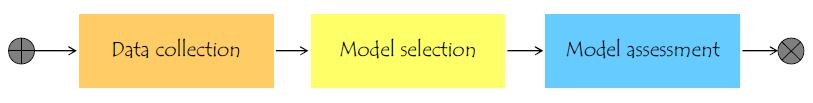
\includegraphics[width=1.0\linewidth]{figures/classification_pipeline}
  \caption{Classification pipeline}
  \label{fig:classificationPipeline}
\end{figure}

\subsection*{Data collection}
Definition of the attributes that describe a data item and the class label. Domain knowledge is needed to know which attributes are relevant for the classification task.

As shown on Figure \ref{fig:dataCollection}, here are the different step in our data collection pipeline:
\begin{enumerate}
	\item Definition of the features that describe a data item
	\item Label the data items to create a training set
	\item Discretisation of the features
	\item Selection of the relevant features
	\item Normalisation of the features
\end{enumerate}

\begin{figure}[!ht]
  \centering
  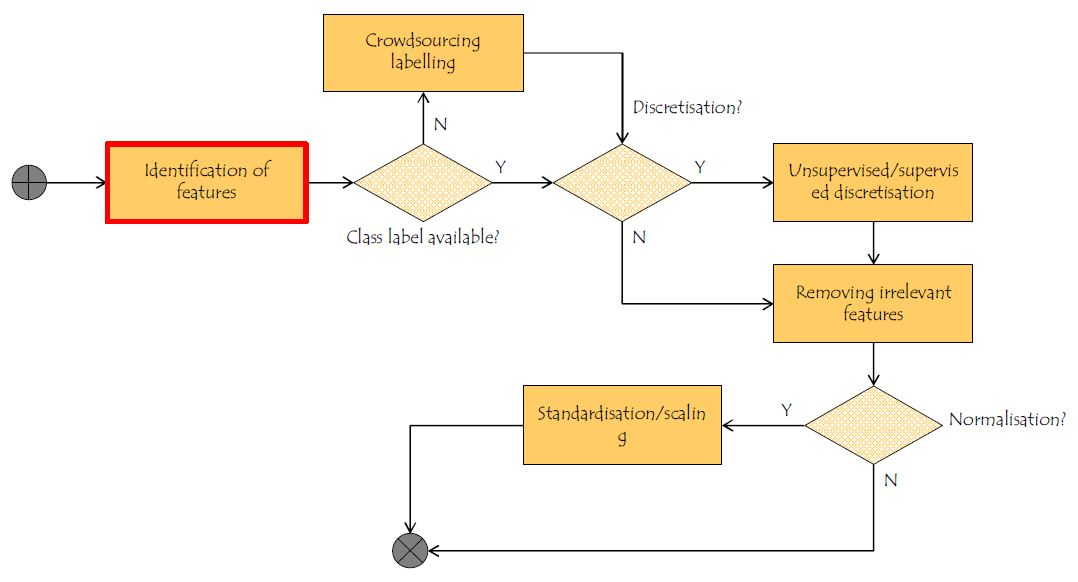
\includegraphics[width=1.0\linewidth]{figures/data_collection}
  \caption{Data collection pipeline}
  \label{fig:dataCollection}
\end{figure}

There exist different types of features:
\begin{itemize}
	\item Numerical (e.g., age, temperature)
	\item Ordinal (e.g., phone code, ...)
	\item Categorical (e.g., student, animals, ...)
\end{itemize}

It is easy to collect data on the web but difficult to label them. The basic idea of crowdsourcing is to enroll a large group of people that will contribute to a specific task. It suits really well for labelling a large data set. However, some of the workers aren't truthful, reliable, and are even sometimes random.

\subsubsection*{Aggregation algorithms}
Given the labelling provided by workers, requester might face the problem of aggregating the answers when they don't coincide.

There are two main classes of aggregation algorithms:
\begin{itemize}
	\item \textbf{Non-iterative}: take the matrix of answers provided by the workers, pre-process it and produce an estimate of the probability that a webpage X is labelled by label L.

	\textbf{Majority decision} algorithm is fast and appropriate for on-line aggregations but very sensitive to spammers. It estimates $P(x_j = l)$ as 
	\begin{align*}
		P(x_j = l) = \frac{1}{N} \sum_{i = 1}^N (1 | a_i(x_j) = j)
	\end{align*}
	with $x_j$ the webpage, $N$ the number of workers, $l$ le label and $a_i(x_j)$ the answer of worker $i$.

	\textbf{Honey pot} algorithm inserts webpages for which the labels are known and will remove workers that fail at correctly labelling more than $m$ of these webpages. It is more robust to spammers but trapping labels are not always available and good workers might be misidentified as spammers if trapping questions are too difficult.

	\item \textbf{Iterative}: take the matrix of answers provided by the worker and produce an estimate of the probability that a webpage X is labelled by label L. With this estimate they update the \textbf{expertise of each worker}, that is, a metric that indicates how good is the worker at performing the labelling task. With this new information, the probability that a webpage X is labelled by label L is estimated again. This cycle continues until convergence.

	\textbf{Expectation Maximisation (EM)} algorithm iterate so as to reduce the expertise of spammers and to increase the expertise of good workers.
	\begin{itemize}
		\item \textbf{E step}: estimate $P(x_j = l)$ as
		\begin{align*}
			P(x_j = l) = \frac{1}{\sum_{i = 1}^N w_i} \sum_{i = 1}^N (w_i | a_i(x_j) = l)
		\end{align*}
		with $w_i$ the expertise weight of worker i

		\item \textbf{M step}: update the expertise $w_i$ as
		\begin{align*}
			w_i = \frac{1}{M} \sum_{j = 1}^M (1 | a_i(x_j) = \argmax_l P(x_j = l))
		\end{align*}
		with $M$ the number of webpages to label
	\end{itemize}

	The EM algorithm is very accurate and very robust to spammers, but slow to converge.
\end{itemize}

\subsubsection*{Discretisation}
\textbf{Unsupervised} discretisation do not take class information into account.
\begin{itemize}
	\item \textbf{Equal width}: divide the range into a predefined number of bins.\\
	$\rightarrow$ lose information is observations are not distributed evenly.
	\item \textbf{Equal frequency}: divide the range into a predefined number of bins so that every interval contains the same number of values.
	$\rightarrow$ many occurences of the same value could be assigned to different bins
	\item \textbf{Clustering}: Perfect for discretisation and can be performed on all the features at the same time.
\end{itemize}

\textbf{Supervised} discretisation take class information into account, measuring the dependency of a discrete interval of values w.r.t the class label. Test that two adjacent intervals of a feature are independent of the class. If they are, merge them.

\subsubsection*{Feature selection}
\textbf{Filtering}: rank features according to their predictive power and select the best ones.
\begin{itemize}
	\item \textbf{Pros}: independent of the classifier
	\item \textbf{Cons}: assume features are independent
\end{itemize}


Correlation coefficient:
\begin{align*}
	r = \frac{\sum_{i = 1}^n (X_i - \bar{X})(Y_i - \bar{Y})}{\sqrt{\sum_{i = 1}^n (X_i - \bar{X})^2} \sqrt{\sum_{i = 1}^n (Y_i - \bar{Y})^2}}
\end{align*}

Mutual information measures the information that $X$ and $Y$ share:
\begin{align*}
	I(F, C) &= H(C) - H(C | F) = H(F) + H(C) - H(F, C)\\
	H(F) &= - \sum_i P(f_i) \log_2 P(f_i)\\
	H(F, C) &= - \sum_i \sum_j P(f_i, c_j) \log_2 P(f_i, c_j)
\end{align*}
If $I(X, Y) = 0$, knowing X does not tell anything about Y.

The chi-square test checks the independence of the class and the feature, without indicating the strength or direction of any existing relationship.

\textbf{Important}: Collectively relevant features may look individually irrelevant.

\textbf{Wrapper}: starts with no features and add the feature that provide the highest improvement in classification accuracy.
\begin{itemize}
	\item \textbf{Pros}: interact with the classifier and no independence assumption
	\item \textbf{Cons}: computationally intensive
\end{itemize}

\subsubsection*{Feature normalisation}
Some classfiers do not manage well features with very different scales.

\textbf{Standardisation}
\[
	x_i' = \frac{(x_i - \mu_i)}{\sigma_i}
\]
with $\mu_i$ the mean value of feature $x_i$ and $\sigma_i$ its standard deviation.
The drawback of this method is that it assumes that data has been generated by a Gaussian process, which is not always true.

\textbf{Scaling}
\[
	x_i' = \frac{x_i - m_i}{M_i - m_i}
\]
with $M_i$ and $m_i$ the max and min values of feature $x_i$ respectively
The drawback of this method is that it doesn't work well with outliers. The "normal" values will be scale to a very small interval.

\subsection{Model selection}
Once the dataset is ready, we have to select the model that provides the best classification accuracy. 

\begin{figure}[!ht]
  \centering
  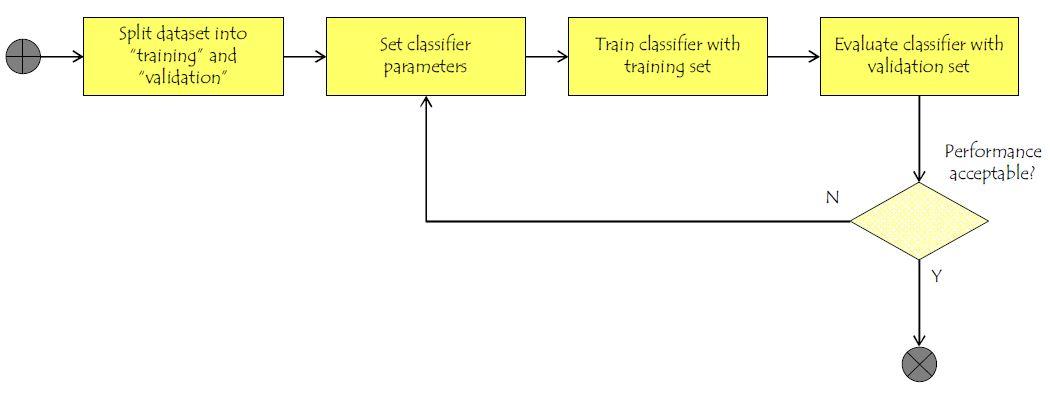
\includegraphics[width=1.0\linewidth]{figures/model_selection}
  \caption{Model selection pipeline}
  \label{fig:modelSelection}
\end{figure}

The task consists in exploring the configuration space of the model in order to find the parameterisation that minimises the loss function.

\begin{itemize}
 	\item \textbf{0-1 loss function} (categorical values)
 	$$ J = \sum_{i = 1}^n \#(y \neq f(x_i)) $$
 	\item \textbf{Squared error} (real values)
 	$$ J = \frac{1}{n} \sum_{i = 1}^n (y_i - f(x_i))^2 $$
 	\item \textbf{Absolute error} (real values)
 	$$ J = \frac{1}{n} \sum_{i = 1}^n |y_i - f(x_i)| $$
 \end{itemize} 

\subsubsection*{Performance metric for Binary Classification}
For categorical binary classification, the usual metrics consider four types of errors as shown on Fig. \ref{fig:binClass}.\\

\begin{figure}[!ht]
  \centering
  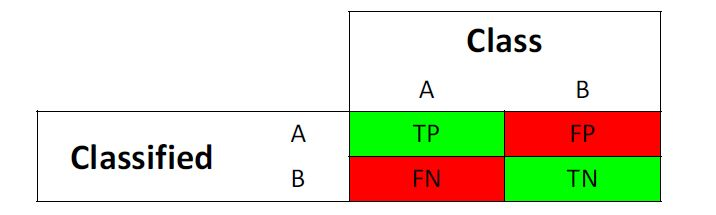
\includegraphics[width=1.0\linewidth]{figures/binary_class}
  \caption{Error types in binary classification}
  \label{fig:binClass}
\end{figure}

\textbf{Accuracy}: the total correct examples divided by the total examples to be classified
$$ A = \frac{TP + TN}{TP + TN + FP + FN} = \frac{TP + TN}{N}$$

\textbf{Precision}: high precision means a few irrelevant examples treates as important
$$ P = \frac{TP}{TP + FP} $$

\textbf{Recall}: high recal means being good at getting the positive class right, fraction of relevant examples that are retrieved.
$$ R = \frac{TP}{TP + FN} $$

\textbf{F-score}: it's necessary to have a unique metrix to compare classifiers.
$$ F1 = 2 \cdot \frac{P \cdot R}{P + R} $$
It is the harmonic mean of precision and recall.

The simplest way to do model selection is constructing a train and validation set. The drawback of this approach is that it does not use all the data to train, and it is possible that the test set is not representative of the classification tasks.

\textbf{Leave-one-out cross validation}
\begin{itemize}
	\item almost unbiased estimate of the true accuracy
	\item time consuming since number of iterations equal number of examples
\end{itemize}

\textbf{K-fold cross validation}: good compromise between having an unbiased estimate and computation time.

\textbf{Bias} and \textbf{variance} can be assessed by comparing the error metrix on the training set and the test set. In the ideal case, we want low bias (small training error) and low variance (small test error). We can observe several cases:
\begin{itemize}
	\item High bias and high variance: worst case
	\item High variance: overfitting $\rightarrow$ should reduce the complexity of the model and add regularisation parameter.
	\item High bias: underfitting $\rightarrow$ should increase complexity of the model and reduce regularisation parameter.
\end{itemize}

\subsection{Model assessment}
Model assessment is the goal of estimating the classification accuracy of a fixed model.

%\afterpage{\null\newpage}



\section{Social Graph}

In social graph mining, we often want to extract significant communities of users.

\subsection{Community evaluation}

Before extracting communities from a social graph, we need to define what is a strong community (well defined) and what is a weak communities (weak bounds between members).

\subsubsection{Strong or weak community}

For a given vertex $i$ we define
\begin{itemize}
  \item the internal degree $k_i^{int}$ the number of edges from $i$ going to another vertex of the community
  \item the external degree $k_i^{ext}$ the number of edges from $i$ going to a vertex outside of the community
\end{itemize}

For a node $i$ correctly assigned to a community $C$, we should have a high $k_i^{int}$ and a low $k_i^{ext}$. More formally

\[
  \sum_{i\in C} k_i^{int}(C) > \sum_{i\in C} k_i^{out}(C)
\]

\subsubsection{Modularity}

Modularity measures how well a graph $G$ is partitioned into communities $S$

\paragraph{Modularity.}
  \[
    Q \propto \sum_{s \in S} (\text{\# edges within } s) - (expected \text{ \# edges within } s)
  \]
  The expected value is computed on a graph with same degree distribution but random connections (null model).


\paragraph{Normalized modularity.}
  \[
    Q(G,S) = \underbrace{\frac 1 {2m}}_{\text{normalize}} \sum_{s\in S, i,j\in s} \l(A_{ij} - \frac{k_ik_j}{2m}\r)
  \]
  and $-1<Q<1$


Modularity is positive if the intra connection exceeds the expected number. A partitioning is significant if $Q>0.3,0.7$. We can use modularity to know when to stop community extraction algorithm (pick).

\subsection{Community extraction}

% We build a similarity matrix ($A_{ij}$ how node $i$ and $j$ are similar) from the adjacency matrix.

Hierarchical clustering algorithms identifies groups of nodes with high similarity. We can distinguish two strategies:

\begin{itemize}
  \item \textbf{Agglomerative algorithm:} merge nodes and communities with high similarity
  \item \textbf{Divisive algorithm:} split communities by removing links connecting nodes with low similarity (smallest cut)
\end{itemize}

In both strategy, we need a stopping point for the iterative process. Either we chose an arbitrary number of communities $k$ or we use a criteria (see modularity).

\paragraph{Girvan-Newman method.} Divisive hierarchical clustering based on edge betweenness. Iteratively remove edge of highest betweenness. Runs in $O(ln^2)$, $O(n^3)$ for sparse graph.

\paragraph{Louvain Modularity.} Greedy optimization in $O(n\log n)$, find small communities locally and then group smallest communities as simple nodes.

\subsubsection{Edge betweenness}

\paragraph{Edge betweenness.}
  Number of shortest paths passing over an edge (max $n(n-1)$)


\paragraph{Random walk betweenness.}
  Given two nodes $i$ and $j$, $x_{ij}$ is the probability that the edge between $i$ and $j$ is taken by a walk averaged over all the random walks between the pairs of node of the graph.


\subsubsection{How to compute betweenness ?} 

Repeat for each node, but let take $A$ w.l.o.g. (see \cref{fig:betweenness})

\begin{itemize}
  \item BFS from node $A$, all nodes are layered
  \item For each node $i$, count the number of shortest paths arriving to $i$. Recursively sum up the count of the parents (assigning 1 to node $A$).
  \item Assign edge values bottom up, each node has value $1 + \sum ($child edges weight$)$, to distribute proportionally to its parents according to their weight
  \item Repeat for each node, sum the weights and divide by two (paths discovered twice - from each end).
\end{itemize}


\begin{figure}
  \centering
  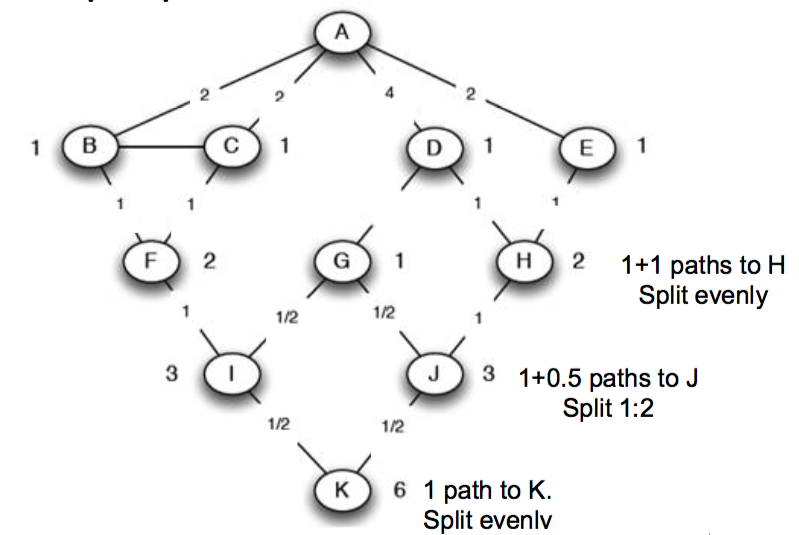
\includegraphics[width=1\linewidth]{figures/betweenness_computation.png}
  \caption{Betweenness computation - BFS, top down node weighting, bottom up edge values}
  \label{fig:betweenness}
\end{figure}

\subsubsection{$k$-medoids for cluster extraction}

We can use $k$-medoids with arbitrary chosen starting centers and a given distance function (weight on the edges for instance). Should start with multiple starting point to avoid being stuck in bad local optimum.

\subsection{Random graphs}

\paragraph{Small world graphs.}
  Graph for which most nodes are not neighbors of one another but most nodes can be reached from any other node by a small number of hops


\paragraph{Milgram's experiment.} Send a message from Nebraska to Massachusetts, from people to friends/relatives (mean of 5-6 hopes)

The experiment rises two problem, how to explain that there exists such short paths in  the social graph, and how to actually find these shortest paths efficiently ?

\subsubsection{Random graph model $G(n,p)$}

Simplest model, take $n$ nodes, connect each pair of nodes with probability $p$. It has the following properties

\begin{itemize}
  \item \textbf{low diameter}, expected distance between two nodes is $\log_k n$ with $k$ the average out degree,
  \item a pair $(i,j) \in V^2$ picked uniformly at random is connected by a short path with high probability
  \item \textbf{low clustering} coefficient (inaccurate for social graph modeling)
\end{itemize}

\paragraph{Diameter.}
  The diameter of a graph $G$ is the longest shortest path between any pair of nodes.

\paragraph{Local clustering coefficient.}
  The local clustering coefficient is the proportion of neighbors connected for a given node. Formally for a given node $i$ with neighbors $N$ and edges between them $E$
  \[
    C_i = \frac { 2|E|}{|N|(|N|-1)}
  \]

\paragraph{Global clustering coefficient.}
  Average of the local clustering coefficient.
  \[
    C = \frac 1 n \sum_i^n C_i
  \]

\subsubsection{Watts and Strogatz model}

Random rewiring of regular graph: take a regular graph and with probability $p$ rewire each link to a randomly selected node. Resulting graph has properties, both of regular and random graphs, see \cref{fig:watts_strogatz}.

\begin{figure}
  \centering
  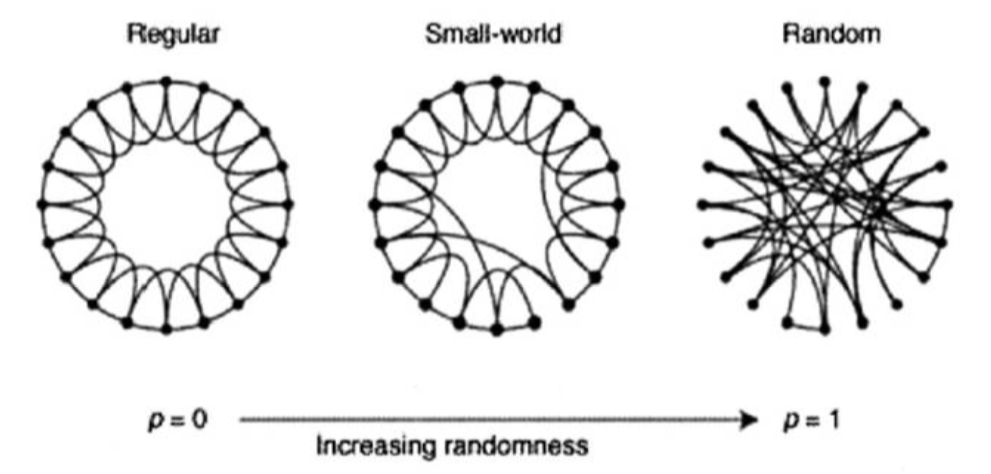
\includegraphics[width=1\linewidth]{figures/watts_strogatz_graph.png}
  \caption{Watts Strogatz rewiring construction}
  \label{fig:watts_strogatz}
\end{figure}

\subsubsection{Efficient search algorithm (Kleinberg’s model)}

\begin{itemize}
  \item Embed a graph into an $d$-dimensional grid to define a distance function ($l$2 norm for instance)
  \item each node is connected to $p$ of its closest neighbor (short range links) + $q$ random nodes (long range links) according to a distribution
  \[
    \P{u \leftrightarrow v} \propto \text{dist}(u,v)^{-r}
  \]
\end{itemize}

Decentralized routing algorithm performs well if and only if $r=$ dimension of the space. If $r$ is too small, we go far but struggle to converge, if $r$ is too high we stay among our neighbors, hard to reach the neighborhood of the target.

For $r=0$ we chose the long range links uniformly, like a random graph. there exist short paths between every pair of vertex but there is no decentralized algorithm capable of finding these paths efficiently.

\paragraph{Routing cost.} With $O(1)$ long range link $O(\log^2 n)$, and with $O(\log n)$ long range links $O(\log n)$.



\section{Recommender systems}

\paragraph{Definition.} Given a user and a set of items, a recommender system is a function that helps to match users with items by ranking the items in order of decreasing relevance.

We can discern two paradigms for recommender systems: 
\begin{itemize}
  \item \textbf{Collaborative:} tell me what other people like
  \item \textbf{Content-based:} show me more of what I liked from my past ratings and the data of these objects
\end{itemize}

\subsection{Collaborative user based filtering}

Widely used by large e-commerce sites, applicable in many domains. Users give ratings to items, we assume that users with similar tastes in the past will have similar tastes in the future.

\paragraph{Problems.} Cold start, scalability, more users than items (huge neighborhood), data dispersion (hard to find neighborhood). Possible solution: compute predictions offline and use learned model online + update model regularly.

\paragraph{Technique.} Given a user $U$ and an item $I$ not rated by $U$, estimate the rating $r_U(I)$

\begin{enumerate}
  \item Find a set of users $N_u$ who liked the same items as $U$ in the past and who have rated $I$
  \item Aggregate the ratings of $I$ provided by $N_U$ to get $r_U(I)$
  \item Compute the ratings for all the items not rated by $U$ and recommend the best-rated ones 
\end{enumerate}

\subsubsection{Similarity metric}
We need a metric to compute similarity between users and find the closest neighborhood of a user. 

\paragraph{Pearson correlation coefficient} as similarity measure. Given two users $x$ and $y$, a set of items $I$ rated by both $x$ and $y$ ($|I| = N$), and $r_x(i)$ the rating of $x$ for $i\in I$, the Pearson correlation coefficient is given by
\[
  \text{sim}_{corr}(x,y) = \frac {\sum_{i=1}^N (r_x(i)-\bar r_x)(r_y(i) - \bar r_y) } { \sqrt {\sum_{i=1}^N (r_x(i) - \bar r_x)^2} \sqrt {\sum_{i=1}^N (r_y(i) - \bar r_y)^2}}
\]
We have $-1 \leq \text{sim}(x,y) \leq 1$


\paragraph{Cosine similarity.} It consider each user as a $N$ length vector and compute the angle between $\mathbf{x}$ and $\mathbf{y}$. If angle is 0 the two ratings are very close (sim returns 1), if the vetors are orthogonal it return 0.

\[
  \text{sim}_{cos}(x,y) = \frac {\sum_{i=1}^N r_x(i)r_y(i)}{\sqrt{\sum_{i=1}^N r_x(i)^2} \sqrt{\sum_{i=1}^N r_y(i)^2}}
\]

One drawback of Pearson correlation coefficient is that it is not computable if the variance of one of the user ratings is 0 (e.g. a user with ratings 1 1 1 1). However, in general, the correlation coefficient works well in usual domains, compared to the cosine similarity. The reason is that the cosine similarity does not consider the magnitude of the ratings but only the angle between the vectors.

\subsubsection{Aggregate the ratings}

The following aggregation function is a weighted average using the similarity as a weight

\[
  r_x(a) = \bar r_x + \frac {\sum_{y \in N_x} \text{sim}(x,y)(r_y(a) - \bar r_y)} {\sum_{y \in N_x} |\text{sim}(x,y)|}
\]

\subsection{Item-based collaborative filtering}

We use the similarity between items (and not users) to make predictions. Given a user $U$ and an item $I$ not rated by $U$, estimate the rating $r_U(I)$:

\begin{enumerate}
  \item Find a set of items $N_I$ who are similar to $I$ and that have been rated by $U$
  \item Aggregate the ratings of the items in $N_I$ and use the aggregation as prediction of $r_U(I)$
\end{enumerate}

Be careful that in this technique the similarity between objects is computed only with regard to the rating given by users (two objects are similar if they have been graded the same way by the users). We don't use the content/description of the object (yet).

\paragraph{Aggregate the ratings.}

\[
  r_x(a) = \frac{\sum_{b\in N_a} \text{sim}(a,b) r_x(b)}{\sum_{b\in N_a} |\text{sim}(a,b)|}
\]

There is still the scalability problem but we can calculate all the pair-wise item similarities in advance. Items similarities are more stable and we only need to consider the neighborhood (small) at runtime.

\subsection{Content-based recommendation}

\begin{enumerate}
  \item Find the items that are similar to the past rated items
  \item Aggregate the ratings of the most similar items
\end{enumerate}

The content of an item is often noisy if input by the manufacturer and hard to compare between the items, a formalism is needed to compute the similarity.

\paragraph{TF-IDF weights} For textual description, we can use this technique to describe a text by the set of terms that appear in their description, with their associated weight. Given $N$ the number of items and $n(t)$ the number of items having word $t$ in their description

\[
  w(t,a) = \text{tf}(t,a) \cdot \text{idf}(t) = \frac{\text{freq}(t,a)}{\max_{s\in T} \text{freq}(s,a)}\log\pfrac N {n(t)}
\]

To compute the TF-IDF measure, all the steps typical of information retrieval (removing stopwords, stemming, only top M terms etc.) are necessary.

\paragraph{Cosine similarity.} Given $1 \dots T$ the terms appearing in all the items,

\[
  \text{sim}_{cos}(a,b) = \frac {\sum_{t=1}^T w(t,a)\cdot w(t,b)}{\sqrt{\sum_{t=1}^T w(t,a)^2}\sqrt{\sum_{t=1}^T w(t,b)^2}}
\]

\paragraph{Aggregation.} For a given item $a$ not rated yet, we have neighbor items $N_a$ rated by the user we make a prediction by the following formula

\[
  r_x(a) = \frac {\sum_{b\in N_a} \text{sim}(a,b) \cdot r_x(b)}{\sum_{b\in N_a} | \text{sim}(a,b)|}
\]

\paragraph{Problems.} Cold start, content can be limited or impossible to extract (multimedia), tends to recommend “more of the same”. Advantage: TF-IDF scores can be computed offline.

\subsection{Netflix Prize}

What we need to know:

\begin{itemize}
  \item Input of the challenge: utility matrix, try to guess the grey part (see \cref{fig:netflix_matrix})
  \item Winners: BellKor and Ensemble, code never used in production
  \item Ensemble is a mixing of models of different former teams
\end{itemize}

\begin{figure}
  \centering
  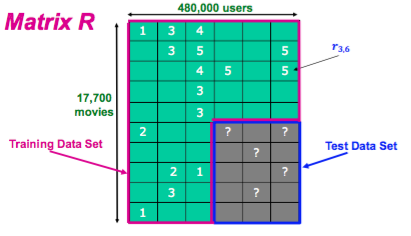
\includegraphics[width=1\linewidth]{figures/netflix_matrix.png}
  \caption{Netflix utility matrix}
  \label{fig:netflix_matrix}
\end{figure}

\paragraph{Bellkor solution.} Multi-scale modeling of the data
\begin{itemize}
  \item Global: mean rating overall users plus average difference of the user, to have a baseline
  \item Factorization: address regional effect
  \item Local neighborhood: related movies
  \item An idea is to embed the movies in a multi dimension vector space: Latent Factor Models (e.g. SVD)
\end{itemize}


\end{document}
